% !TEX encoding = UTF-8 Unicode
\documentclass[hyperref={bookmarks=false}]{beamer}
\usetheme{CambridgeUS}
\setbeamercolor{bibliography entry author}{fg=black}
\setbeamercolor{item}{fg=darkred}
\setbeamercolor{caption name}{fg=darkred}
\beamertemplatenavigationsymbolsempty

\usepackage[serbianc]{babel}
\usepackage{type1ec}
\usepackage{cmap}

\graphicspath{{../slike}}
\newcommand{\lenitem}[2][.43\linewidth]{\parbox[t]{#1}{\strut #2\strut}}

\title[\textit{HMM} у биоинформатици]{Скривени Марковљеви модели у биоинформатици -- електронска лекција}
\titlegraphic{
\includegraphics[height=2.9cm,width=3.5cm]{matf2.png}}
\author[Лазар Васовић]{Студент: Лазар Васовић\\ Ментор: Јована Ковачевић}
\date[Математички факултет]{23. септембар 2021.}

\begin{document}

\frame{\titlepage}

\begin{frame}{Садржај}
\tableofcontents[subsectionstyle=hide]
\end{frame}

\section{Увод}
\subsection{Биоинформатика}
\begin{frame}{Биоинформатика}
\mbox{}\hfill\raisebox{-\height}[0pt][30pt]{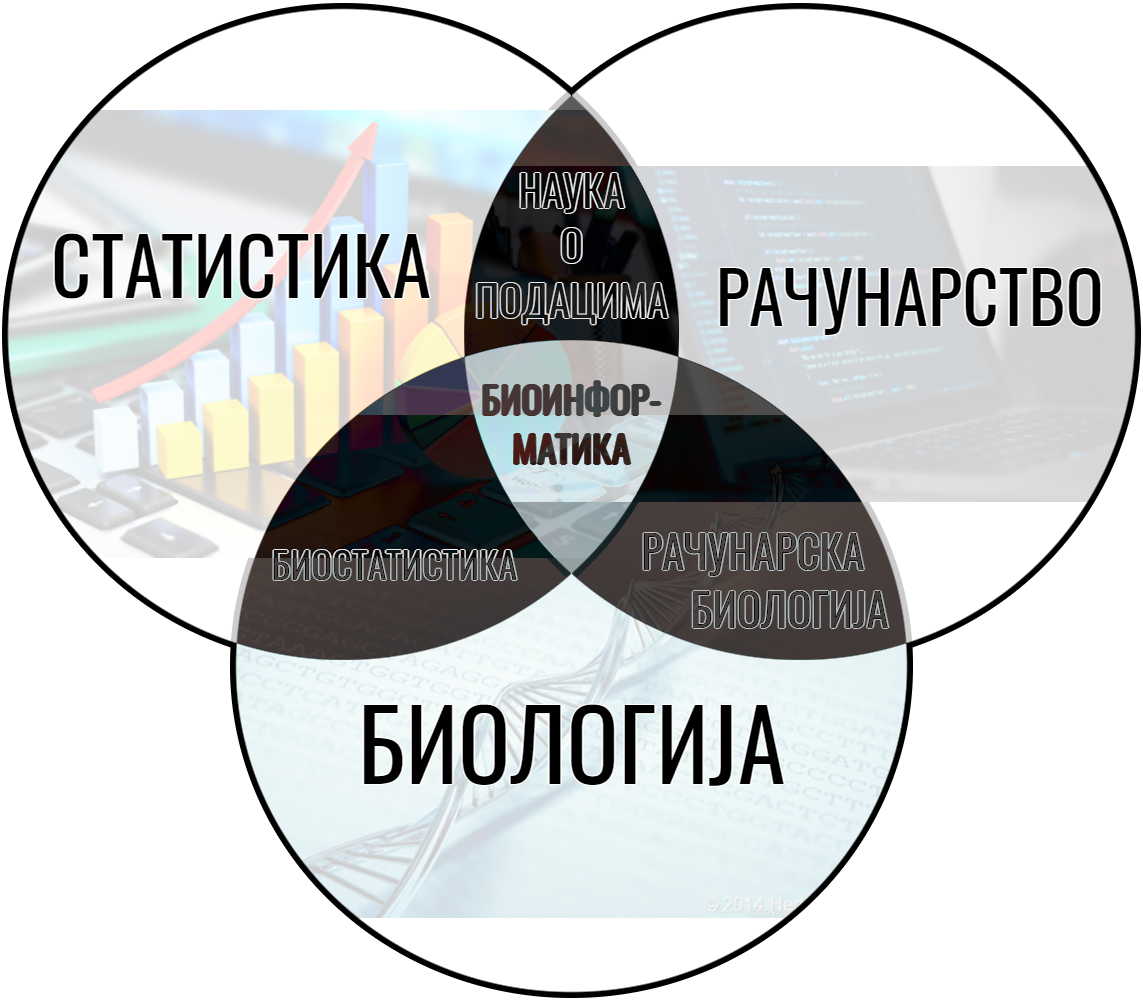
\includegraphics[width=.5\linewidth]{bioinformatika.png}}
\vspace*{-\baselineskip}

\begin{itemize}
\item \lenitem{Биоинформатика је интердисциплинарна област која се бави применом рачунарских технологија у области биологије и сродних наука, са нагласком на разумевању биолошких података.}
\end{itemize}
\end{frame}

\subsection{Скривени Марковљев модел}
\begin{frame}{Скривени Марковљев модел}
\mbox{}\hfill\raisebox{-\height}[0pt][20pt]{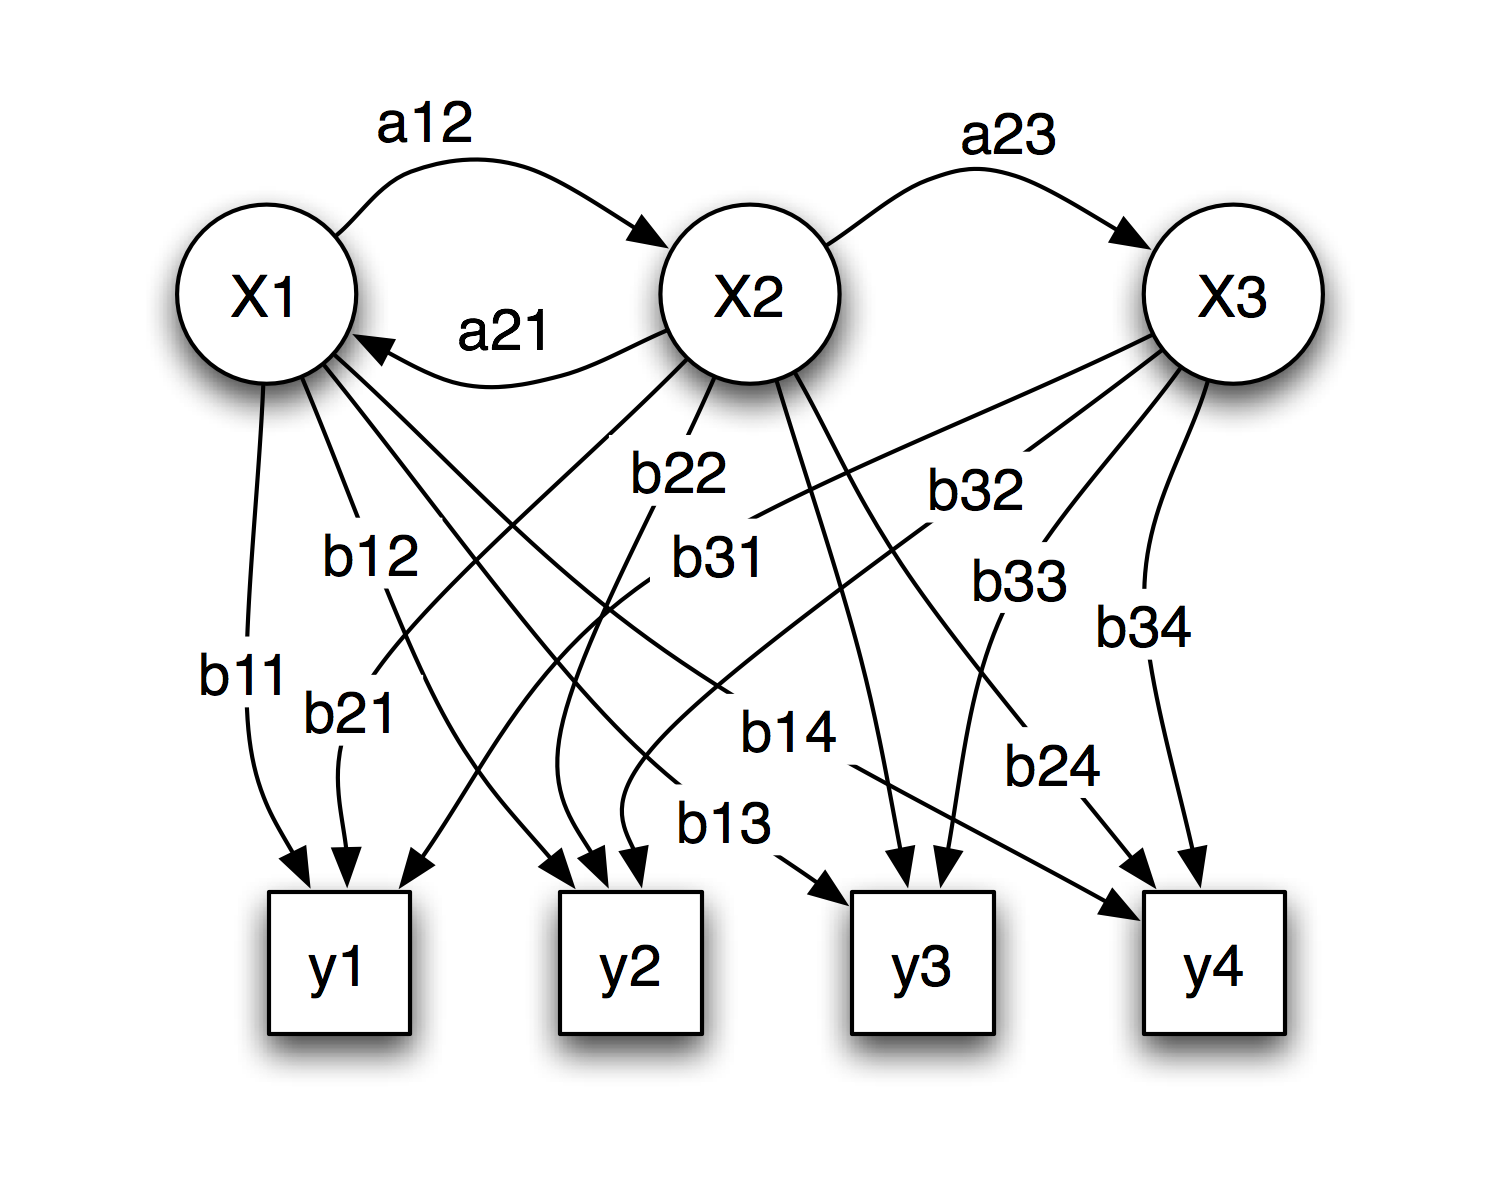
\includegraphics[width=.5\linewidth]{hmm.png}}
\vspace*{-\baselineskip}

\begin{itemize}
\item \lenitem{Скривени Марковљев модел (\textit{HMM}, према енгл. \textit{Hidden Markov Model}) представља вероватносни модел који се састоји из следећих елемената: скривених стања ($x_i$), опсервација ($y_i$), вероватноћа прелаза ($a_{ij}$), полазних ($\pi_i$) и излазних вероватноћа ($b_{ij}$).}
\end{itemize}
\end{frame}

\subsection{Електронска лекција}
\begin{frame}{Електронска лекција}
\mbox{}\hfill\raisebox{-\height}[0pt][20pt]{
\includegraphics[width=.35\linewidth]{jupyter.png}}
\vspace*{-\baselineskip}

\begin{itemize}
\item \lenitem{Лекција проширује десето поглавље књиге/уџбеника \textit{Bioinformatics Algorithms: An Active Learning Approach}.}
\item \lenitem{Резултат је \textit{Jupyter} свеска са \textit{Python} кодовима.}
\item \lenitem{Лекција је јавно доступна на \textit{GitHub} репозиторијуму.}
\end{itemize}
\end{frame}

\section{Мотивација}
\subsection{Погађање фенотипа}
\begin{frame}{Погађање фенотипа}
\begin{itemize}
\item Код лечења ХИВ-а, значајно је да ли изолат којим је пацијент заражен ствара синцицијум -- нефункционалну вишеједарну цитоплазматичну масу са заједничком ћелијском мембраном.
\item Испоставља се да је примарна структура гликопротеина омотача \textit{gp120}, конкретно \textit{V3} петље, важан предиктор фенотипа.
\item Електронска лекција -- имплементирано правило 11/25.
\item Проблем је како прецизно лоцирати (поравнати) геном новог изолата, како би правило могло да се примени.
\end{itemize}
\end{frame}

\subsection{Потрага за генима}
\begin{frame}{Потрага за генима}
\begin{itemize}
\item Већина нуклеотида ДНК не кодира протеине, па је један од важних биолошких проблема управо проналажење места на којима се гени налазе.
\item Гене има слисла тражити у стабилним регионима ДНК, који нису подложни метилацији. Такви региони називају се \textit{CG} острвима или \textit{CpG} местима.
\item Електронска лекција -- имплементиран прозорски приступ.
\item Проблем је како одредити ширину прозора и обрадити преклапајуће прозоре.
\end{itemize}
\end{frame}

\subsection{Коцкање са јакузама}
\begin{frame}{Коцкање са јакузама}
\begin{itemize}
\item Једноставан мотивациони пример за увођење \textit{HMM} је непоштена коцкарница -- крупије баца новчић, који у сваком тренутку може бити праведан или отежан (два потенцијална новчића).
\item Могуће је опазити само резултат бацања, а задатак је на основу тога одредити највероватнији низ коришћених новчића.
\item Електронска лекција -- имплементиран прозорски приступ.
\item Проблеми прозорског приступа остају нерешени.
\end{itemize}
\end{frame}

\section{Моделовање}
\subsection{Дефиниција модела}
\begin{frame}{Дефиниција модела}
\begin{itemize}
\item Крупије се, уместо као особа, може схватити као аутомат, за који се испоставља да у потпуности одговара појму скривеног Марковљевог модела, као уређене петорке из увода.
\item Основну дефиницију погодно је надградити, нпр. увођењем експлицитног почетног стања, заменом матрица мапама или употребом логаритмованих вероватноћа.
\item Електронска лекција -- имплементирана класа која представља допуњени \textit{HMM} и приказана њена улога у моделовању непоштене коцкарнице.
\end{itemize}
\end{frame}

\subsection{Могућности модела}
\begin{frame}{Могућности модела}
\begin{itemize}
\item Могуће је дефинисати појам скривеног пута $p = p_1...p_k$ као низ $k$ стања кроз која \textit{HMM} пролази, а да притом емитује секвенцу опсервација $o = o_1...o_k$. Главна идеја је анализирати у ком су односу $p$ и $o$, те са којом се вероватноћом реализују.
\item Једноставним формулама рачунају се вероватноћа пута $P(p) = \prod_{i=1}^k a_{p_{i-1}, p_i}$, вероватноћа $P(o | p) = \prod_{i=1}^k a_{p_{i-1}, p_i} \cdot b_{p_i, o_i}$ исхода на путу, те заједничка вероватноћа пута и исхода $P(p, o) = P(p) P(o | p)$, чијом се максимизацијом за познато $o$ (низ исхода бацања) добија највероватније $p$ (низ новчића).
\item Електронска лекција -- имплементирано израчунавање вероватноћа према формулама и наивна максимизација грубом силом.
\end{itemize}
\end{frame}

\subsection{Витербијев алгоритам}
\begin{frame}{Витербијев алгоритам}
\begin{itemize}
\item Наивни приступ је експоненцијалне сложености, па се максимизацији (декодирању) приступа Витербијевим алгоритмом, техником динамичког програмирања заснованом на Витербијевом графу.
\item Овај граф моделује све путеве кроз \textit{HMM} истовремено, а осмишљен је на основу основног временског својства \textit{HMM}, према коме текуће стање зависи искључиво од првог претходног.
\item Електронска лекција -- имплементирана максимизација претходно разматраних вероватноћа $P(p)$, $P(o | p)$, $P(p, o)$, као и $P(p | o)$.
\end{itemize}
\end{frame}

\subsection{Алгоритам „напред”}
\begin{frame}{Алгоритам „напред”}
\begin{itemize}
\item Могуће је моделовати и појединачну расподелу вероватноће опажања $P(o)$, која једина досад није разматрана.
\item Ако се примети да Витербијев алгоритам израчунава $\max_p P(p, o)$, а да је вероватноћа опажања $P(o) = \sum_p P(p, o)$, лако је закључити како се израчунава $P(o)$ преко Витербијевог графа.
\item Електронска лекција -- имплементирано израчунавање вероватноће $P(o)$ и њена максимизација, као и израчунавање $P(p | o)$, чиме је модел комплетиран.
\end{itemize}
\end{frame}

\section{Биолошки значај}
\subsection{Гени -- два стања}
\begin{frame}{Гени -- два стања}
\mbox{}\hfill\raisebox{-\height}[0pt][15pt]{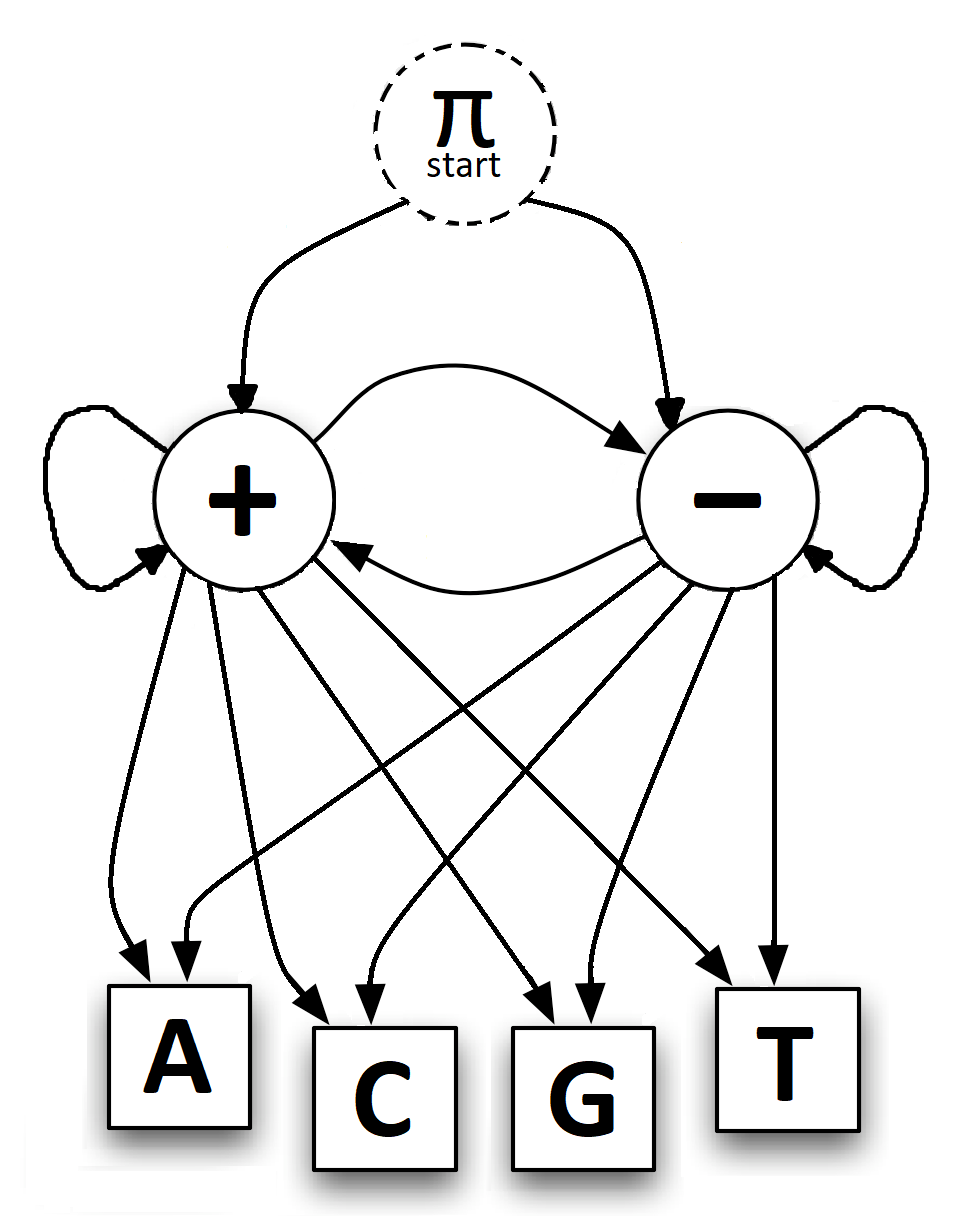
\includegraphics[width=.42\linewidth]{cg_graf.png}}
\vspace*{-\baselineskip}

\begin{itemize}
\item \lenitem{Улазни низ нуклеотида посматра се као секвенца опажања коју треба декодирати.}
\item \lenitem{Параметри модела одређују се на основу знања из генетике или емпиријски.}
\item \lenitem{Најуспешнији је модел који посматра динуклеотиде уместо појединачне симболе.}
\item \lenitem{Електронска лекција -- упоређени различити модели.}
\end{itemize}
\end{frame}

\subsection{Гени -- више стања}
\begin{frame}{Гени -- више стања}
\mbox{}\hfill\raisebox{-\height}[0pt][0pt]{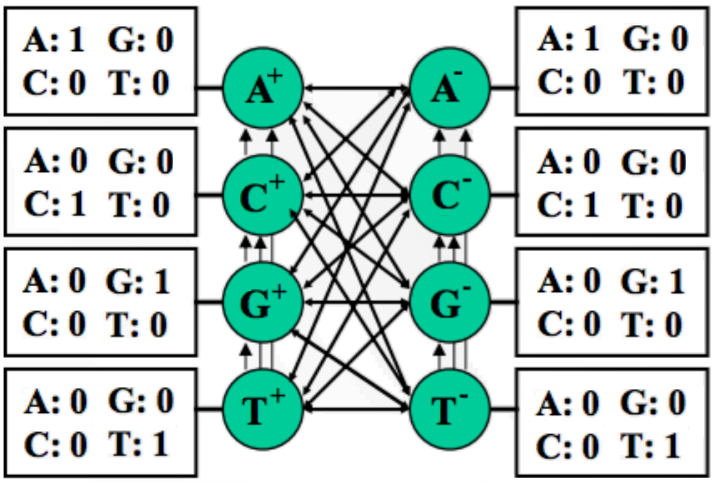
\includegraphics[width=.5\linewidth]{cg_stanja.png}}
\vspace*{-\baselineskip}

\begin{itemize}
\item \lenitem{\textit{CG} острва и региони ван њих могу се моделовати као два одвојена Марковљева ланца, која се могу спојити у \textit{HMM} са осам скривених стања.}
\item \lenitem{Свако стање представља емисију одговарајућег нуклеотида у неком региону.}
\item \lenitem{Електронска лекција -- упоређени различити модели.}
\end{itemize}
\end{frame}

\subsection{Профилни модели}
\begin{frame}{Профилни модели}
\begin{itemize}
\item Протеини су организовани у разнолике протеинске фамилије, а чест биолошки задатак јесте додељивање новооткривеног полипептида некој од познатих фамилија.
\item Користан алат за класификацију протеина јесу профилни \textit{HMM} или \textit{HMM} профили, који статистички описују фамилије протеина, а граде се на основу вишетруког поравнања.
\item Идеја класификације је да се нови полипептиди декодирају профилним моделима неких фамилија, а затим одабере профил у односу на који је вероватноћа припадности изолата највећа или макар прелази предефинисану границу.
\end{itemize}
\end{frame}

\subsection{Рад са профилима}
\begin{frame}{Рад са профилима}
\mbox{}\hfill\raisebox{-\height}[0pt][0pt]{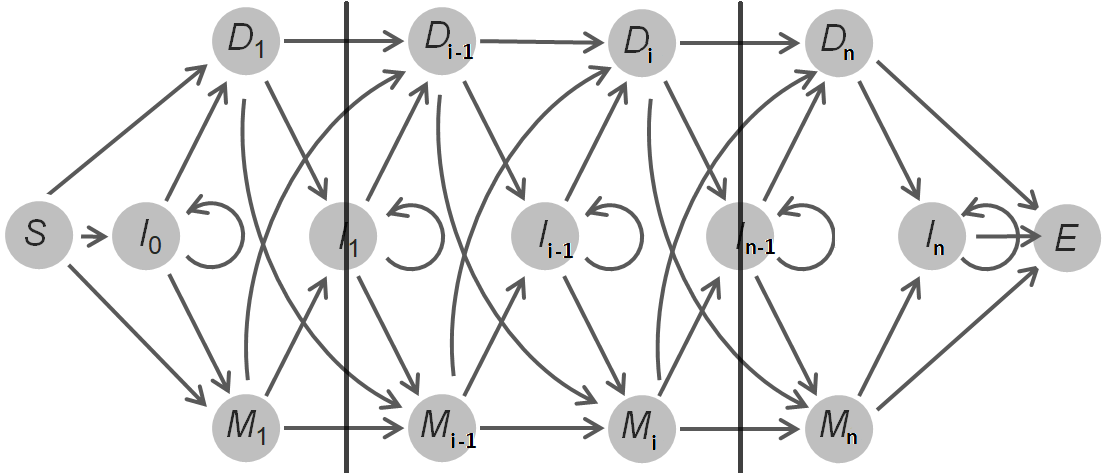
\includegraphics[width=.5\linewidth]{prof_hmm.png}}
\vspace*{-\baselineskip}

\begin{itemize}
\item \lenitem{Профилни \textit{HMM} имају три типа стања, која одговарају мутацијама које настају у геному, уз поклапања.}
\item \lenitem{Параметри модела одређују се емпиријски, по улазном вишеструком поравнању.}
\item Електронска лекција -- имплементирана класа која представља профилни \textit{HMM} и приказана њена улога у раду са секвенцама.
\end{itemize}
\end{frame}

\section{Учење модела}
\subsection{Витербијево учење}
\begin{frame}{Витербијево учење}
\mbox{}\hfill\raisebox{-\height}[0pt][0pt]{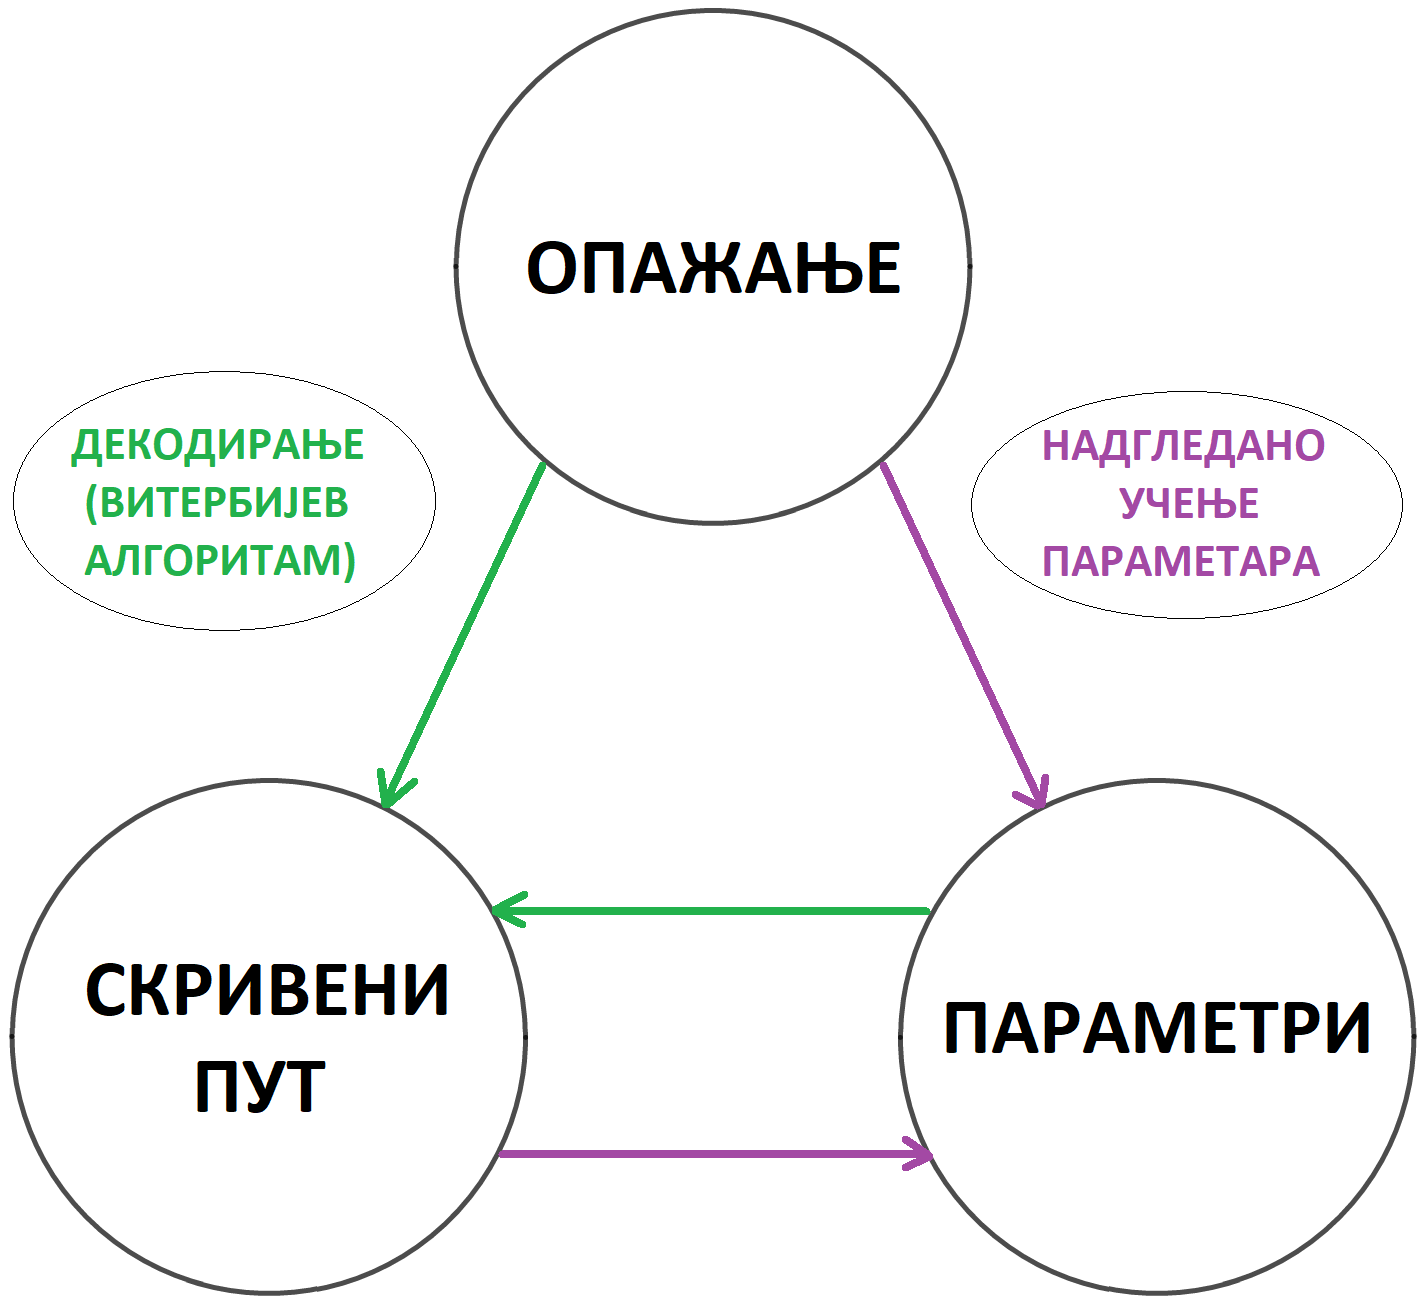
\includegraphics[width=.5\linewidth]{ema.png}}
\vspace*{-\baselineskip}

\begin{itemize}
\item \lenitem{Још једна важна способност \textit{HMM} јесте то да је могуће научити све параметре модела само на основу опажања.}
\item \lenitem{Пре таквог ненадгледаног учења, параметри се могу научити и надгледано (на основу опажања и пута).}
\item \lenitem{Надгледано учење одређује вероватноће на основу фреквенција, док ненадгледано представља алгоритам максимизације очекивања.}
\end{itemize}
\end{frame}

\subsection{Баум-Велчово учење}
\begin{frame}{Баум-Велчово учење}
\begin{itemize}
\item Основна верзија ненадгледаног учења параметара је Витербијево учење, али се чешће користи оптималније Баум-Велчово учење.
\item Декодирање у кораку очекивања мења се новим алгоритмом заснованим на Витербијевом графу: „напред-назад”. Алгоритам одређује вероватноћу да је \textit{HMM} у неком тренутку био у неком скривеном стању.
\item Надгледано учење у кораку максимизације мења се сумирањем одговарајућих индикатора.
\item Електронска лекција -- имплементирани сви типови учења, као и повезани концепти, попут „меког” и апостериорног декодирања.
\end{itemize}
\end{frame}

\section{Закључак}
\subsection{Закључак}
\begin{frame}{Закључак}
\begin{itemize}
\item У раду је изложен појам скривених Марковљевих модела, као и њихов биоинформатички значај. Дата је детаљна мотивација за увођење статистички поткованог аутомата, након чега је појам \textit{HMM} разрађен и примењен на решавање биолошких проблема.
\item Суштински најзначајнији допринос рада је електронска лекција, која, уз детаљну теоријску позадину, садржи и многобројне имплементације. Замисао јој је да допринесе усвајању знања о скривеним Марковљевим моделима и њиховој примени у биоинформатици, а притом буде јавно и свима доступна.
\end{itemize}
\end{frame}

\subsection{Захвалница}
\begin{frame}
\centering \LARGE
\textbf{ХВАЛА НА ПАЖЊИ!}

\textbf{Питања?}
\end{frame}

\subsection{Библиографија}
\begin{frame}{Библиографија}
\nocite{*}
\bibliographystyle{amsalpha}
\bibliography{prezentacija}
\end{frame}

\end{document}